\documentclass[12pt]{article}
\usepackage[a4paper, margin=1in]{geometry}
\usepackage{graphicx}
\usepackage{amsmath}
\usepackage{float}
\usepackage{caption}
\usepackage{subcaption}
\usepackage{hyperref}

\title{\textbf{Disparity Map}}
\author{Niladri Ghosh \\
ID-B2430100 \\
Department of Computer Science }
\date{\today}

\begin{document}

\maketitle

\begin{abstract}
This report presents the implementation of disparity map estimation using stereo image pairs. The disparity map is a crucial component in stereo vision systems, allowing depth perception by analyzing the pixel differences between the left and right images. This project uses OpenCV's StereoBM (Block Matching) and StereoSGBM (Semi-Global Block Matching) algorithms for disparity computation. The report compares both methods and visualizes the output disparity maps.
\end{abstract}

\section{Introduction}
Stereo vision enables the estimation of depth from two images taken from slightly different viewpoints. The difference in position of an object in both images is known as \textit{disparity}, which can be inversely related to depth. This project implements:
\begin{itemize}
    \item Preprocessing of stereo image pairs.
    \item Disparity estimation using StereoBM and StereoSGBM.
    \item Visualization of resulting disparity maps.
\end{itemize}

\section{Methodology}

\subsection{Loading and Preprocessing}
The stereo image pair is loaded in grayscale, which is a prerequisite for disparity computation.

\begin{verbatim}
imgL = cv2.imread('left.png', 0)
imgR = cv2.imread('right.png', 0)
\end{verbatim}

\begin{figure}[H]
    \centering
    \begin{subfigure}[b]{0.45\textwidth}
        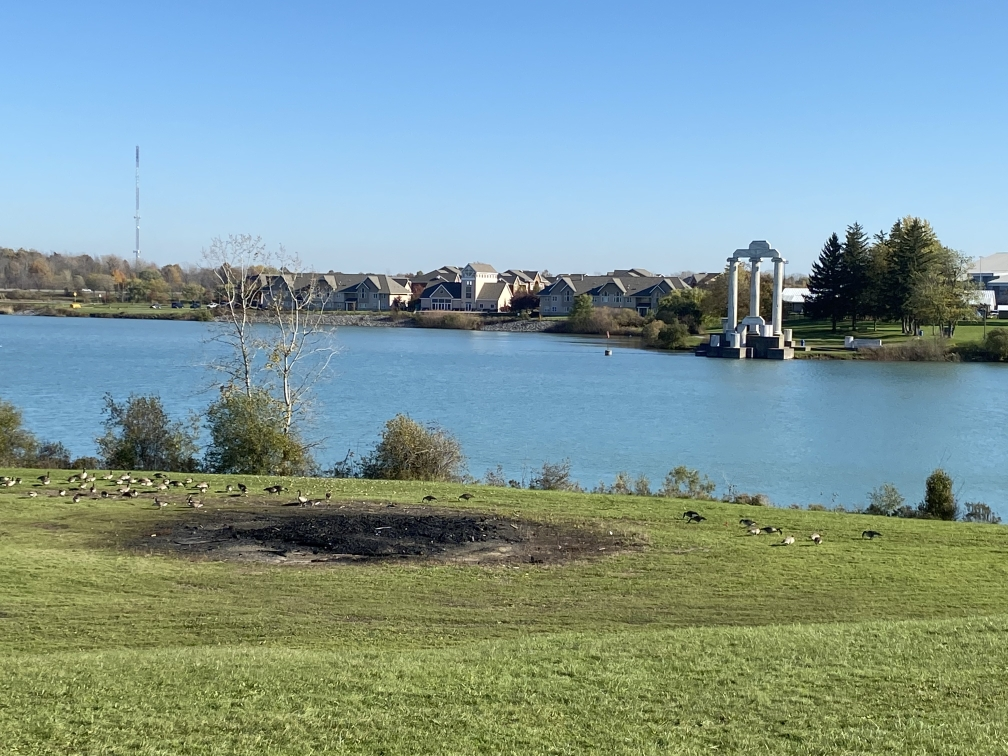
\includegraphics[width=\textwidth]{left.jpg}
        \caption{Left Image}
    \end{subfigure}
    \hfill
    \begin{subfigure}[b]{0.45\textwidth}
        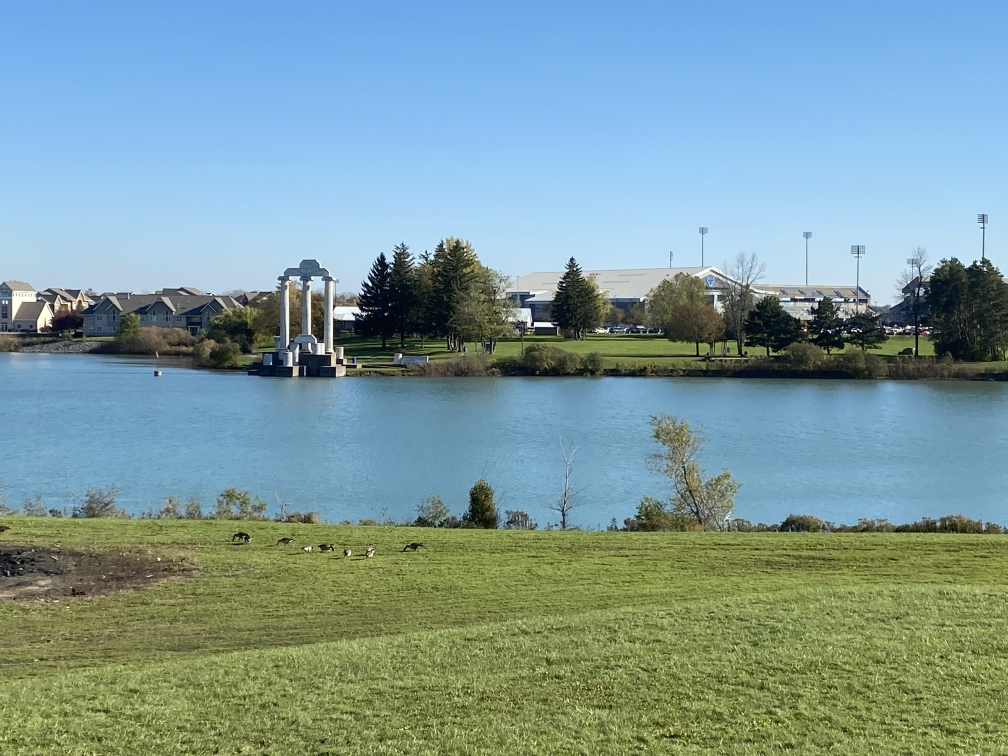
\includegraphics[width=\textwidth]{right.jpg}
        \caption{Right Image}
    \end{subfigure}
    \caption{Stereo Image Pair 1}
\end{figure}

\subsection{Disparity Map using StereoBM}
StereoBM is a traditional block matching algorithm. It's fast and suitable for real-time applications, but may be less accurate in textureless or complex regions.

\begin{verbatim}
stereo = cv2.StereoBM_create(numDisparities=16, blockSize=15)
disparity = stereo.compute(imgL, imgR)
\end{verbatim}


\subsection{Disparity Map using StereoSGBM}
StereoSGBM provides improved accuracy by considering pixel relationships across multiple directions.

\begin{verbatim}
stereo = cv2.StereoSGBM_create(
    numDisparities=16,
    blockSize=5,
    P1=8*3*5**2,
    P2=32*3*5**2,
    disp12MaxDiff=1,
    uniquenessRatio=15,
    speckleWindowSize=50,
    speckleRange=2
)
disparity = stereo.compute(imgL, imgR)
\end{verbatim}

\begin{figure}[H]
    \centering
    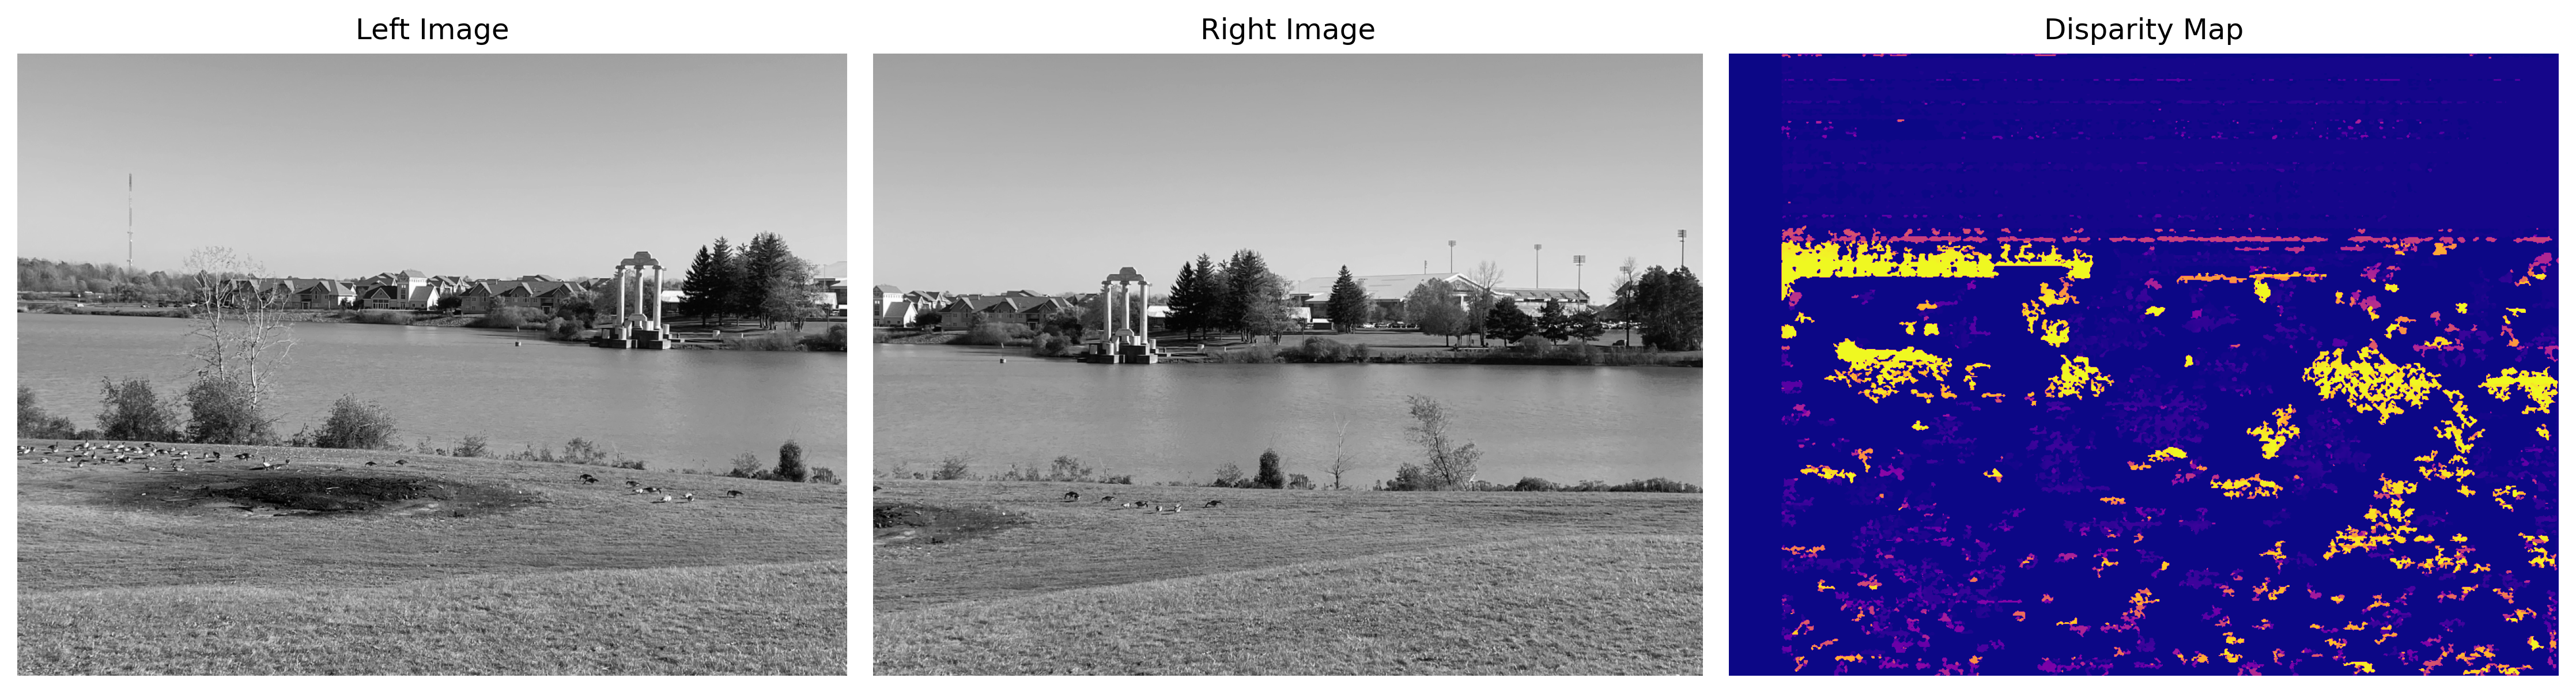
\includegraphics[width=0.8\textwidth]{disparity_result2.png}
    \caption{Disparity Map}
\end{figure}

\section{Results and Analysis}
Both disparity maps successfully highlight depth differences in the scene. Key observations:
\begin{itemize}

    \item \textbf{StereoSGBM}: More refined and accurate at the cost of computation time.
\end{itemize}

I have implemented by taking 2 pictures here is the result:
\begin{figure}[H]
    \centering
    \begin{subfigure}[b]{0.45\textwidth}
        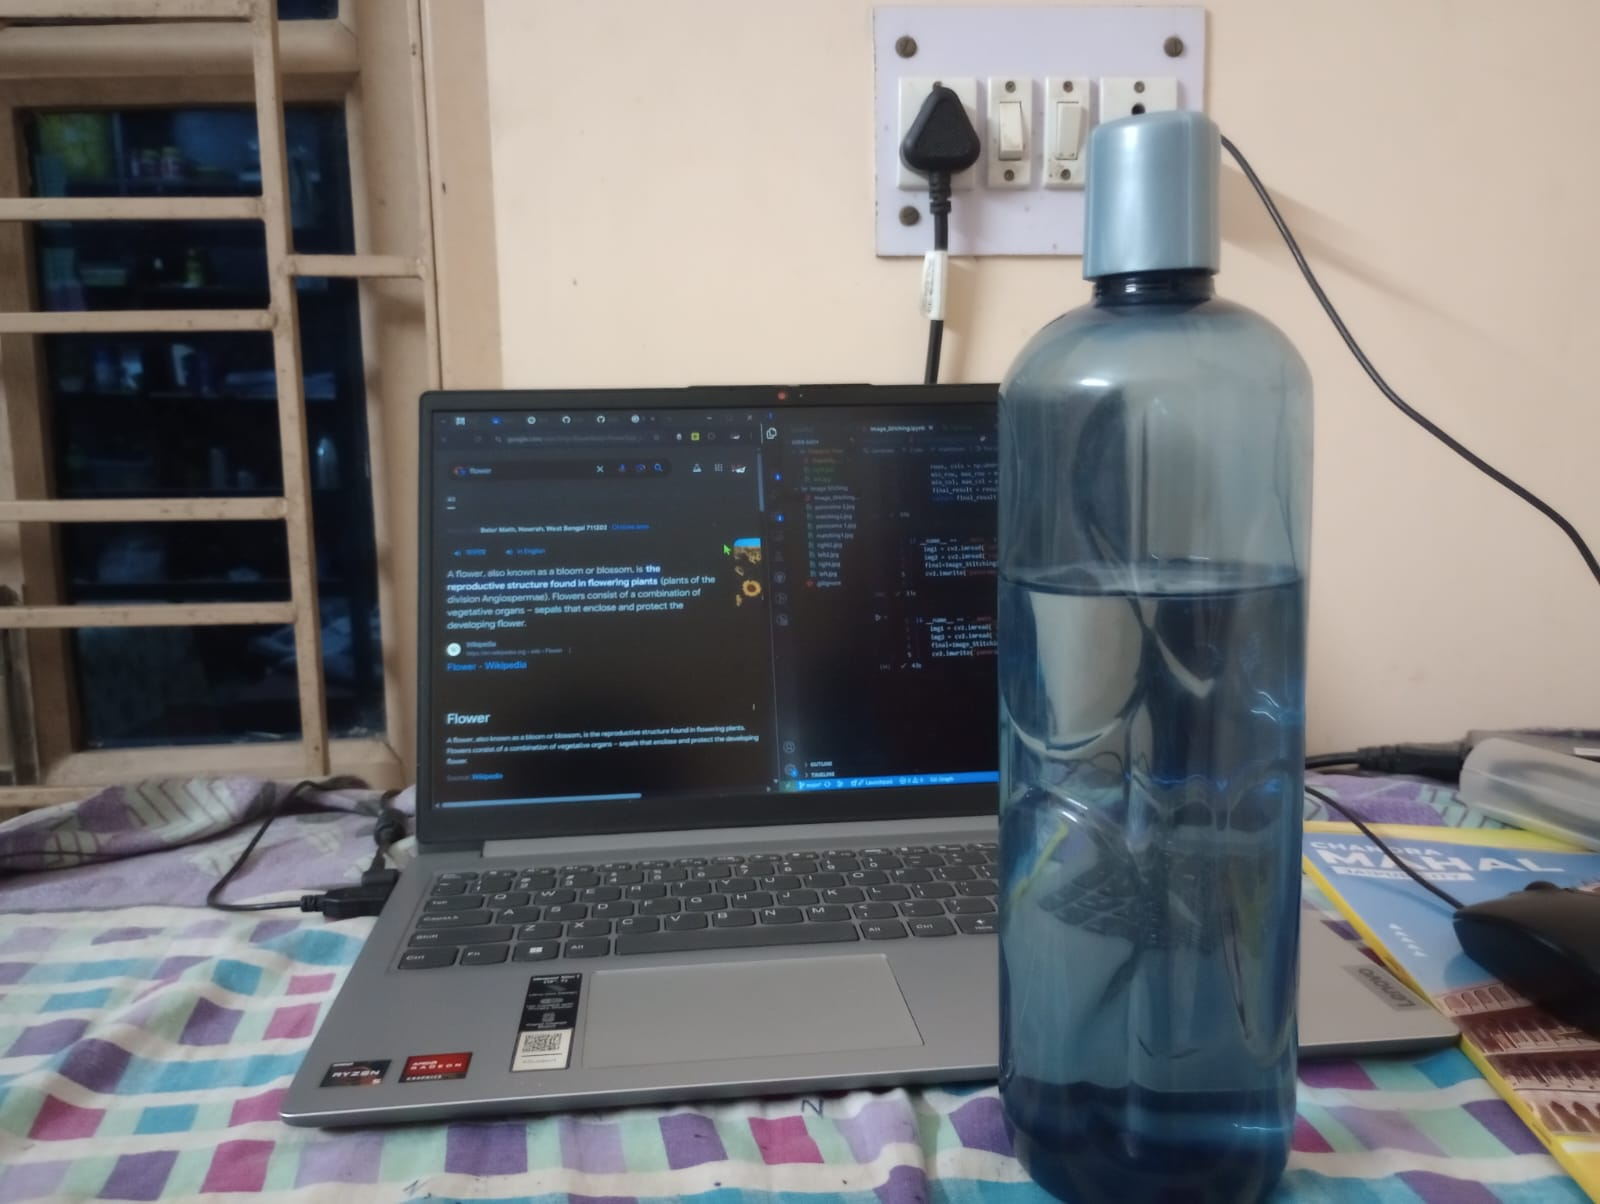
\includegraphics[width=\textwidth]{left2.jpg}
        \caption{Left Image}
    \end{subfigure}
    \hfill
    \begin{subfigure}[b]{0.45\textwidth}
        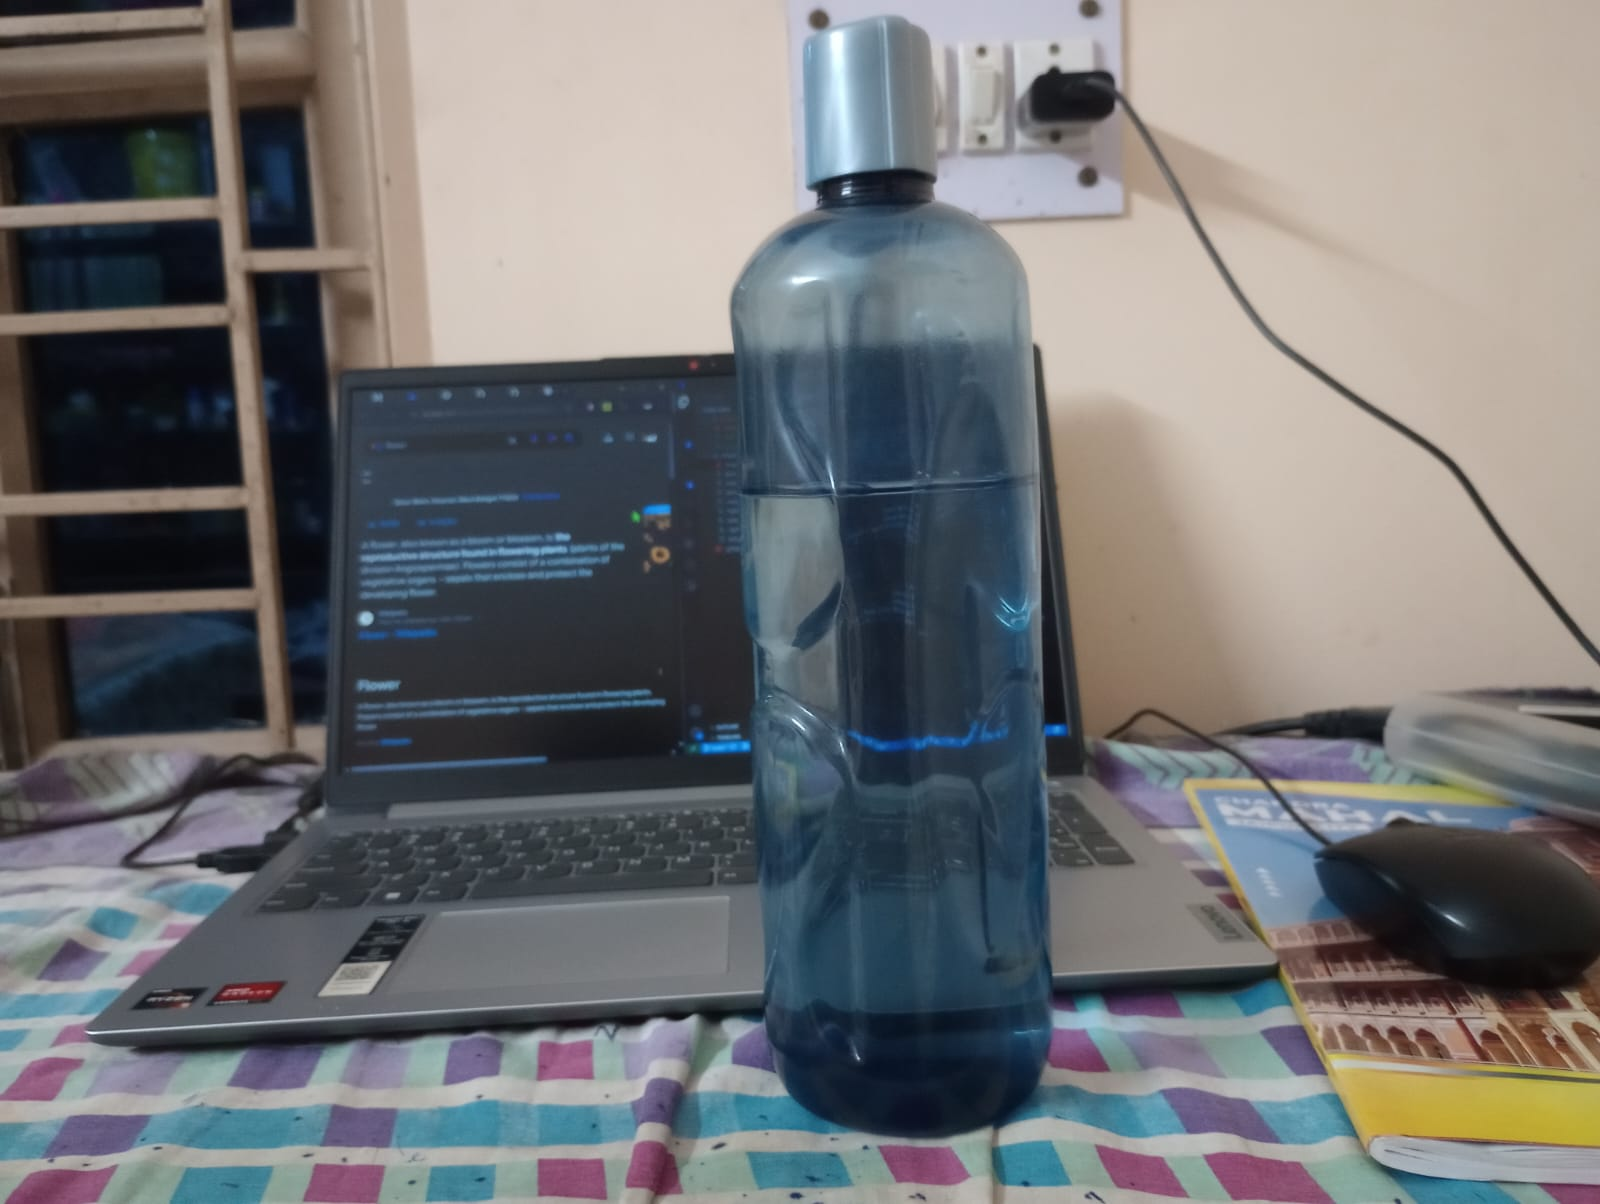
\includegraphics[width=\textwidth]{right2.jpg}
        \caption{Right Image}
    \end{subfigure}
    \caption{Stereo Image Pair 2}
\end{figure}
\begin{figure}[H]
    \centering
    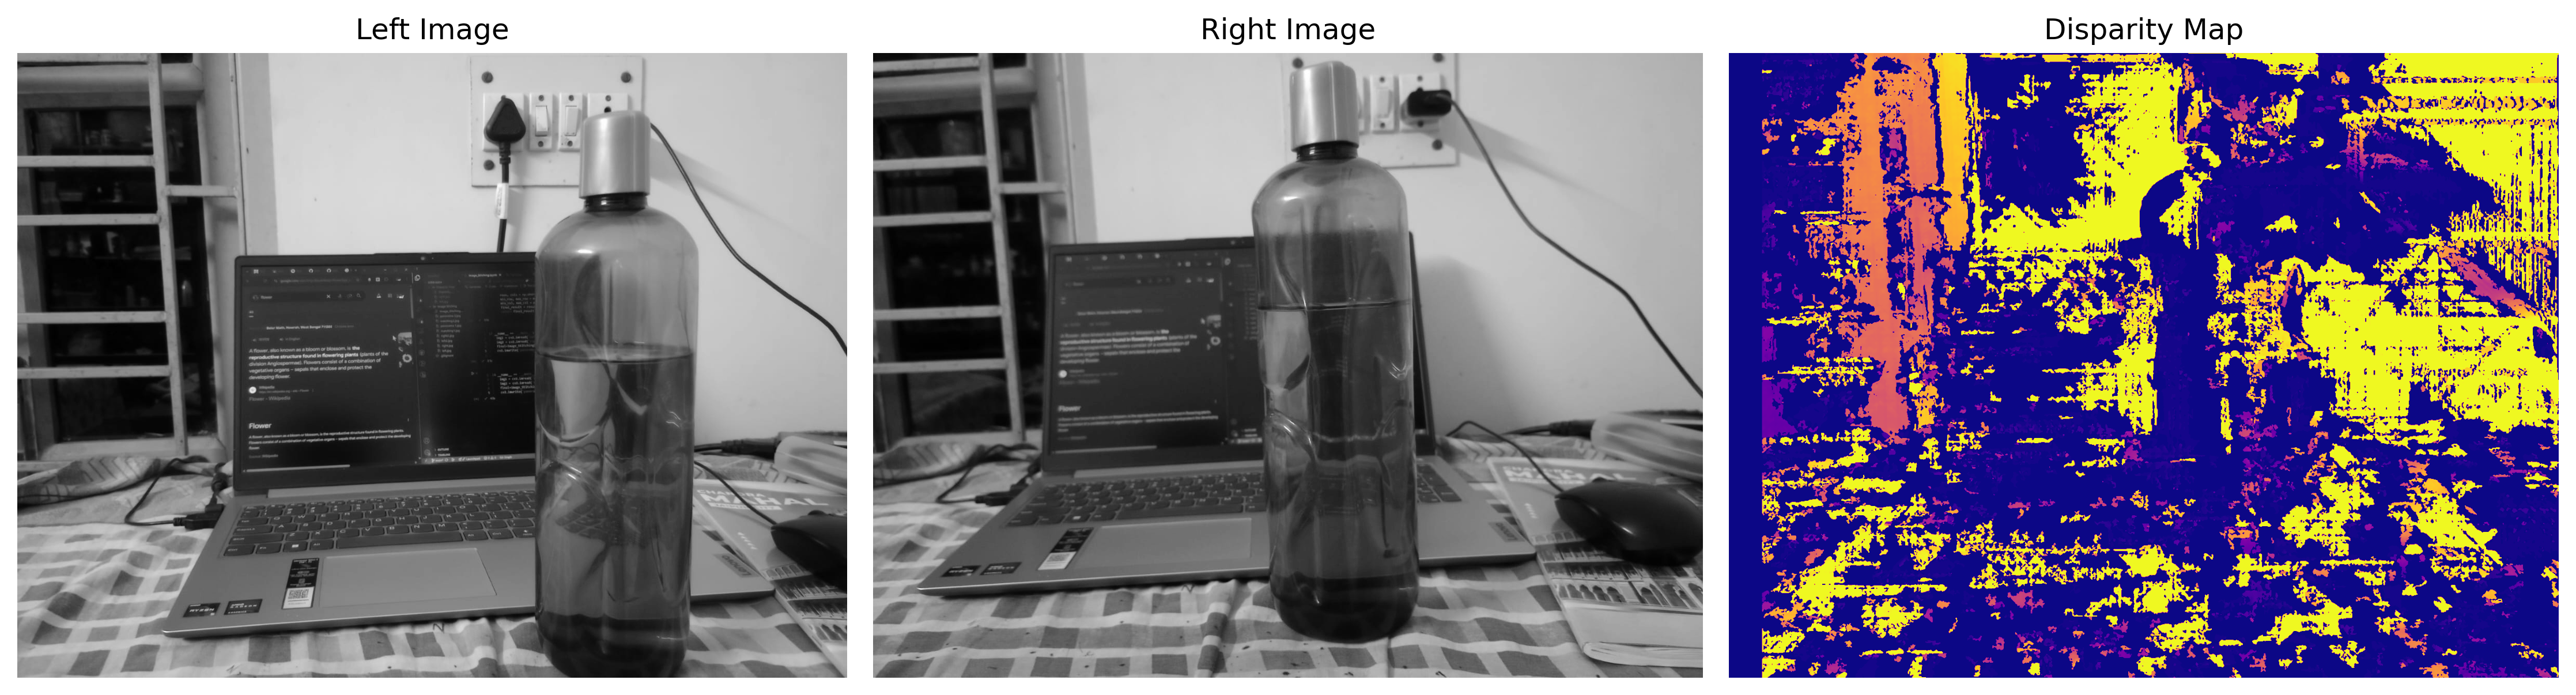
\includegraphics[width=0.8\textwidth]{disparity_result.png}
    \caption{Disparity Map}
\end{figure}

\section{Conclusion}
This project demonstrates two core algorithms in stereo vision—StereoBM and StereoSGBM—for disparity estimation. The disparity map provides a depth representation, which is vital in autonomous navigation, robotics, and 3D reconstruction.

\section{Future Work}
\begin{itemize}
    \item Implement real-time video disparity estimation.
    \item Experiment with custom calibration and rectification for better alignment.
    \item Use machine learning-based stereo matching for superior accuracy.
\end{itemize}

\end{document}
